\documentclass[10pt,twocolumn]{article}

\usepackage[a4paper,margin=0.72in]{geometry}
\usepackage{graphicx}
\usepackage{booktabs}
\usepackage{tabularx}
\usepackage{amsmath}
\usepackage{amssymb}
\usepackage{multirow}
\usepackage{url}
\usepackage{xcolor}
\usepackage{caption}
\usepackage{subcaption}
\usepackage{tikz}
\usepackage{enumitem}
\usepackage{needspace}
\usepackage{placeins}
\usepackage{dblfloatfix}
\usepackage{hyperref}

\captionsetup{font=small,labelfont=bf}
\setlist[itemize]{noitemsep,topsep=2pt,leftmargin=*}
\setlength{\tabcolsep}{4pt}
\renewcommand{\arraystretch}{1.08}
\raggedbottom
\setcounter{topnumber}{3}
\setcounter{bottomnumber}{2}
\setcounter{totalnumber}{4}
\setcounter{dbltopnumber}{2}
\renewcommand{\topfraction}{0.85}
\renewcommand{\bottomfraction}{0.65}
\renewcommand{\textfraction}{0.15}
\renewcommand{\floatpagefraction}{0.60}
\renewcommand{\dbltopfraction}{0.85}
\renewcommand{\dblfloatpagefraction}{0.60}

\hypersetup{
    colorlinks=true,
    linkcolor=blue!55!black,
    citecolor=blue!55!black,
    urlcolor=blue!55!black
}

\title{\vspace{-1.1cm}Low-Light Image Enhancement with Cross-Dataset Generalization}
\author{Giovanni Felle}
\date{}

\begin{document}
\maketitle

\begin{abstract}
This report presents a compact and reproducible deep learning pipeline for low-light image enhancement (LLIE), with emphasis on cross-dataset generalization. A lightweight U-Net baseline is trained on paired LOL-v2 Real Captured images and evaluated in-domain on LOL-v2, cross-domain on LOL-v1, and without reference on ExDark. We compare the baseline against two controlled variants: a ResidualUNet architectural variant inspired by Res-Unet generators, and a training-objective variant that keeps the U-Net architecture unchanged but adds a color constancy term to mitigate color cast. The results show that ResidualUNet improves in-domain PSNR on LOL-v2, while the baseline remains more robust on out-of-domain ExDark. The color-aware loss provides the clearest mitigation for color cast: it keeps PSNR/SSIM nearly unchanged while substantially improving no-reference quality scores and visibly reducing grayish desaturation. A dedicated failure taxonomy analyzes color cast, halo artifacts, over-smoothing, hallucinated details, and residual noise, with causal hypotheses and mitigation strategies.
\end{abstract}

\section{Introduction}
Low-light image enhancement aims to transform underexposed images into visually usable and structurally faithful outputs. A useful LLIE model should not merely brighten the input: it should preserve color balance, recover meaningful structures, avoid amplifying noise, and remain stable when evaluated outside the training distribution. This last point is central to the assignment: the model is trained on one source domain and tested on different datasets.

The project follows a supervised image-to-image restoration protocol. The source domain is LOL-v2 Real Captured, which provides paired low-light and normal-light images. Cross-dataset behavior is tested on LOL-v1 and ExDark. The implementation is intentionally compact: the objective is not to reproduce a large state-of-the-art method, but to build a transparent baseline, a controlled architectural variant, and a targeted mitigation for an observed failure mode.

The main contributions of this first version are:
\begin{itemize}
    \item a reproducible U-Net baseline trained with L1 and SSIM supervision;
    \item a ResidualUNet architectural variant replacing plain convolutional blocks with residual blocks;
    \item a U-Net training-objective variant using a color constancy loss term as a concrete mitigation for color cast;
    \item a cross-dataset evaluation protocol using PSNR, SSIM, NIQE, and BRISQUE;
    \item a qualitative failure taxonomy with causal hypotheses and mitigation discussion.
\end{itemize}

\section{Datasets and Licensing}
\subsection{Datasets}
Three public datasets are used.

\textbf{LOL-v2 Real Captured.} LOL-v2 is used as the source domain for training and validation, and its official test set is used for in-domain evaluation. The project uses the Real Captured subset introduced with the semi-supervised LLIE work of Yang et al.~\cite{yang2020semisupervised}. Each sample contains a low-light input and a normal-light target.

\textbf{LOL-v1 eval15.} LOL-v1 is used as a paired cross-dataset test set. It contains 15 low/normal image pairs and originates from the RetinexNet dataset release~\cite{wei2018retinexnet}. It is useful because it shares the LLIE task definition but differs in dataset construction and image statistics.

\textbf{ExDark.} ExDark is used as an unpaired robustness test~\cite{loh2019exdark}. It contains low-light images across object categories and illumination conditions, but no normal-light ground truth for enhancement. Therefore only no-reference metrics and qualitative analysis are reported. The full dataset is not used as a benchmark in this project: instead, a deterministic stratified subset of 120 images is selected, with 10 images from each of the 12 ExDark categories. This choice keeps evaluation time manageable, preserves category balance, and is intended for robustness and qualitative failure analysis rather than for claiming a complete ExDark benchmark result.

\begin{table}[!htbp]
\centering
\caption{Dataset protocol used in the experiments.}
\label{tab:datasets}
\small
\resizebox{\columnwidth}{!}{%
\begin{tabular}{llr}
\toprule
Dataset & Role & Samples \\
\midrule
LOL-v2 Real train split & Training & 586 \\
LOL-v2 Real val split & Validation & 103 \\
LOL-v2 official test & In-domain paired test & 100 \\
LOL-v1 eval15 & Cross-domain paired test & 15 \\
ExDark stratified split & Cross-domain unpaired test & 120 \\
\bottomrule
\end{tabular}
}
\end{table}

\subsection{Licensing and Terms of Use}
The datasets are not redistributed with this repository. They are expected under \texttt{data/raw/}. The report cites the original dataset papers and release pages. LOL-v2 is associated with the CVPR 2020 semi-supervised low-light enhancement work and dataset release. LOL-v1 is associated with the BMVC 2018 LOL dataset introduced for RetinexNet. ExDark is released through the Exclusively Dark Image Dataset repository. In this project, the data are used only for academic experimentation and are not versioned or redistributed.

\section{Preprocessing}
All images are converted to RGB, resized to $256 \times 256$, and normalized to the $[0,1]$ range. The training split uses seed-controlled random cropping after resizing to \texttt{image\_size + crop\_padding}, horizontal flipping with probability $0.5$, and mild brightness/contrast jitter applied only to the low-light input. These operations follow the standard idea of image data augmentation: increasing the variability of the training distribution through label-preserving geometric and photometric perturbations~\cite{krizhevsky2012imagenet,shorten2019augmentation}. In this paired restoration setting, crop and flip are applied synchronously to the low-light input and the ground truth, so the pair remains spatially aligned. Validation and test transforms are deterministic.

Examples of the actual training augmentation pipeline are shown in Fig.~\ref{fig:augmentation_examples}. The ``VAL transform'' panels show the deterministic resize-only reference, while the ``TRAIN augmented'' panels show the sample after the same training transform used by the data loader.

The current configuration is summarized in Table~\ref{tab:config}. The selected resolution follows the assignment recommendation and keeps training feasible on local hardware. Batch size 8 was chosen as a stable value for Apple MPS memory. \texttt{num\_workers=0} was used because multiprocessing data loading on macOS/MPS can introduce shared-memory overhead and instability; with this small dataset, single-process loading was sufficiently stable.

\begin{figure*}[!tbp]
\centering
\begin{subfigure}[t]{0.48\textwidth}
\centering
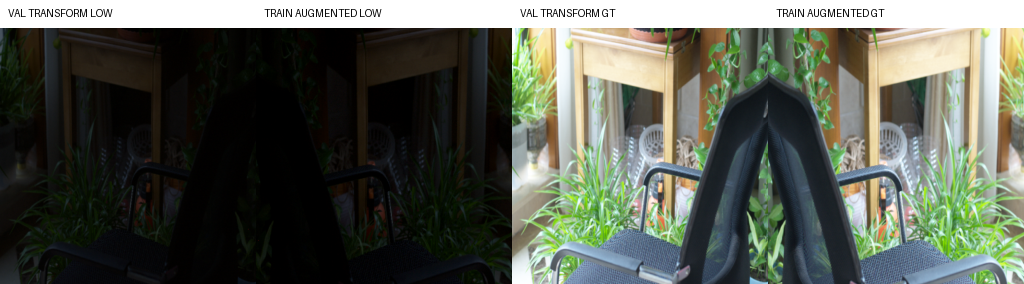
\includegraphics[width=\linewidth]{images/augmentation_003.png}
\end{subfigure}
\hfill
\begin{subfigure}[t]{0.48\textwidth}
\centering
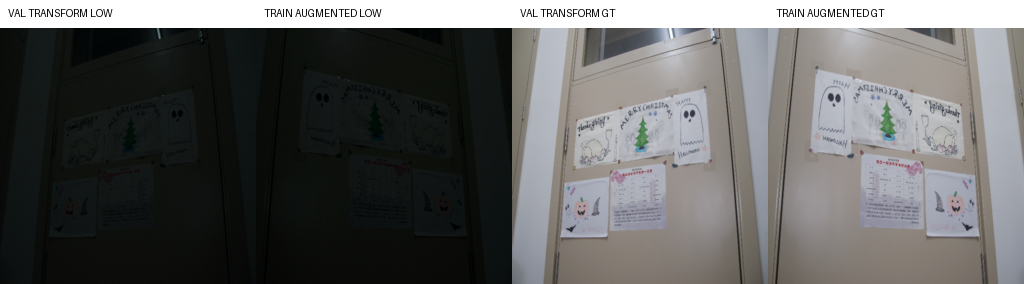
\includegraphics[width=\linewidth]{images/augmentation_004.png}
\end{subfigure}
\caption{Examples of the implemented data augmentation pipeline. The augmented low-light image receives the same crop and horizontal flip as the ground truth, while brightness/contrast jitter is applied only to the low-light input.}
\label{fig:augmentation_examples}
\end{figure*}

\begin{table}[!htbp]
\centering
\caption{Main configuration values.}
\label{tab:config}
\small
\resizebox{\columnwidth}{!}{%
\begin{tabular}{ll}
\toprule
Parameter & Value \\
\midrule
Image size & $256 \times 256$ \\
Batch size & 8 \\
Optimizer & AdamW \\
Learning rate & $3 \cdot 10^{-4}$ \\
Weight decay & $10^{-5}$ \\
Epoch budget & 100 \\
Early stopping patience & 10 \\
Seed & 42 \\
Mixed precision & auto, CUDA only \\
Augmentation & crop, flip, brightness/contrast jitter \\
\bottomrule
\end{tabular}
}
\end{table}

\section{Models}
\subsection{Baseline U-Net}
The baseline is a compact U-Net encoder-decoder inspired by the original U-Net design~\cite{ronneberger2015unet}. Each stage uses a \texttt{DoubleConv} block:
\[
\mathrm{Conv}_{3 \times 3} \rightarrow \mathrm{ReLU} \rightarrow
\mathrm{Conv}_{3 \times 3} \rightarrow \mathrm{ReLU}.
\]
Downsampling is performed with max pooling, upsampling with transposed convolution, and encoder features are concatenated with decoder features through standard U-Net skip connections. The final layer is a $1 \times 1$ convolution followed by a sigmoid, ensuring output pixels remain in $[0,1]$.

The baseline is intentionally simple. This makes it easier to isolate the effect of later changes and to understand whether observed failures arise from the data, the loss, or the model capacity.

\subsection{ResidualUNet Variant}
The architectural variant replaces every \texttt{DoubleConv} block with a residual block, following the residual-learning principle introduced by He et al.~\cite{he2016resnet}:
\[
\mathrm{ResidualBlock}(x) =
\mathrm{ReLU}(F(x) + P(x)),
\]
where $F(x)$ is a two-convolution branch and $P(x)$ is either the identity mapping or a $1 \times 1$ projection when the channel count changes. The network keeps the same high-level U-Net topology as the baseline: encoder, bottleneck, decoder, and skip concatenations.

This design was inspired by the Res-Unet generator proposed by Xiang et al. \cite{xiang2018resunet}. Their work combines U-Net skip connections with residual blocks to improve image synthesis while keeping training efficient. We do not reproduce their GAN or medical cross-modality setting; instead, we adapt the architectural principle to a paired LLIE restoration task. The reference Figure \ref{fig:resunet_arch} supplied with the assignment discussion illustrates the Res-Unet idea: convolutional blocks are augmented with element-wise residual additions, shown in Figure \ref{fig:resblock}, while U-Net skip connections preserve multi-scale information.

Batch normalization was intentionally omitted in our ResidualUNet and in our baseline U-Net. Low-light enhancement depends on preserving absolute intensity and color statistics. BatchNorm normalizes feature distributions using mini-batch statistics; with a small batch size of 8, these statistics can be noisy and may introduce luminance or chromatic shifts between training and inference. Since color fidelity is a central failure mode in this project, we avoid normalization.

\begin{figure*}[!tbp]
\centering
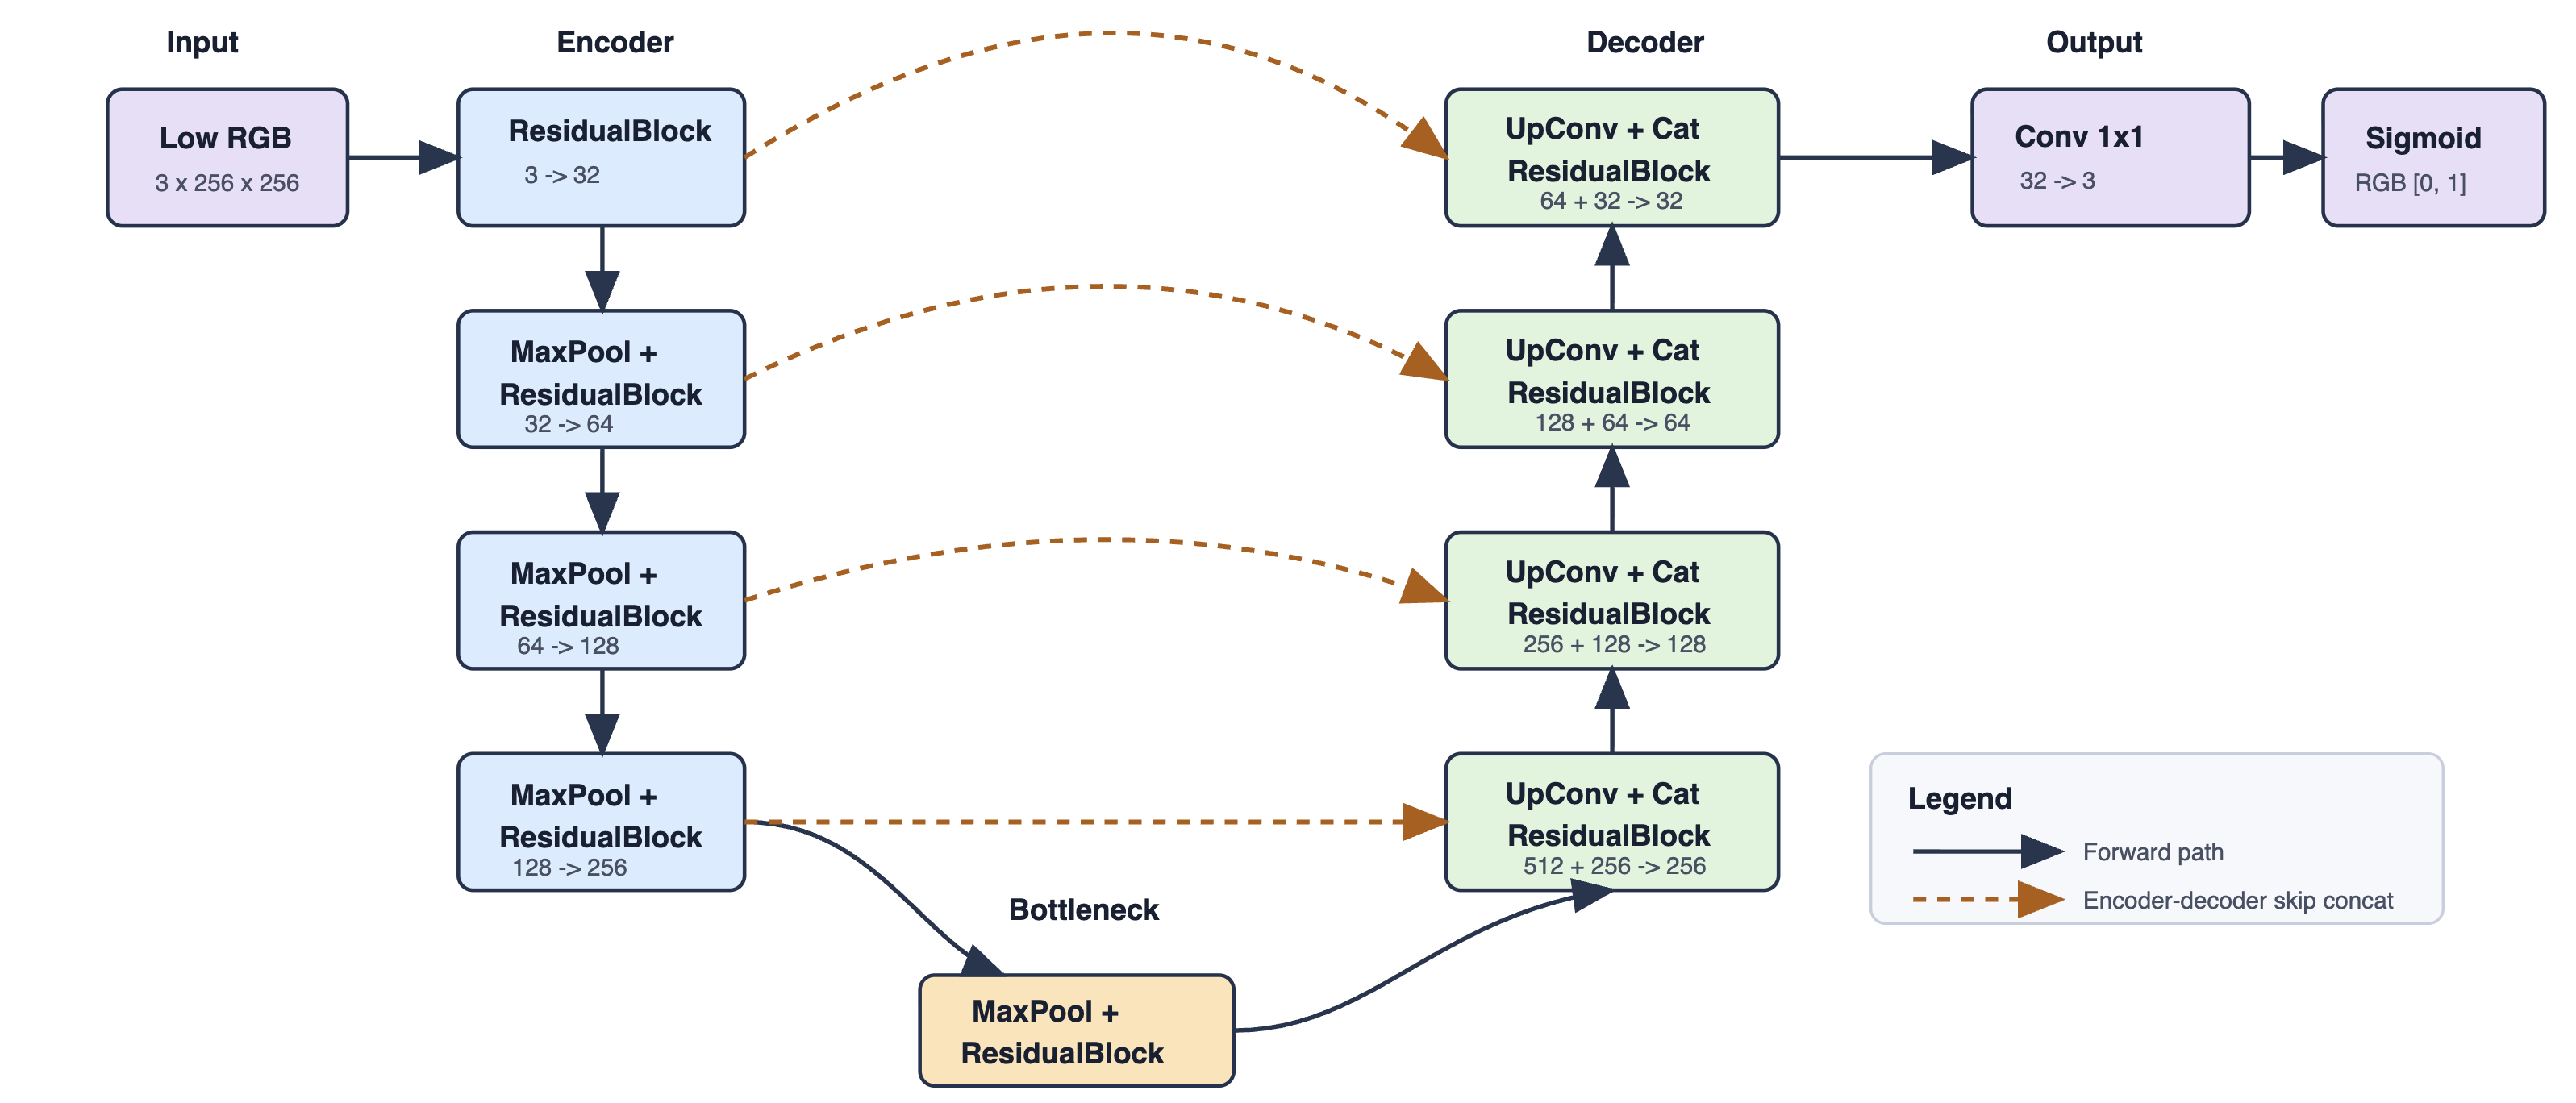
\includegraphics[width=0.96\textwidth]{images/residual_unet_architecture.png}
\caption{Implemented ResidualUNet architecture. The variant keeps the U-Net encoder-decoder structure but replaces DoubleConv modules with residual blocks. Dashed arrows indicate encoder-decoder concatenation skips.}
\label{fig:resunet_arch}
\end{figure*}

\begin{figure}[!htbp]
\centering
\resizebox{0.95\columnwidth}{!}{
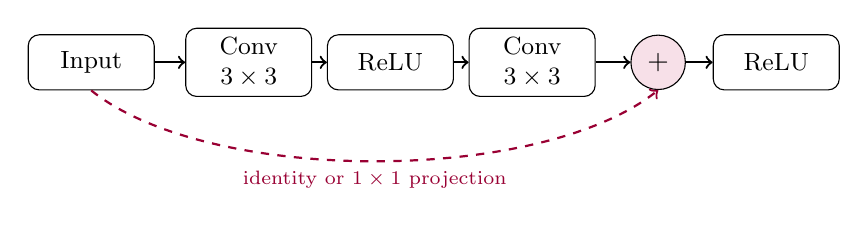
\begin{tikzpicture}[
    block/.style={draw, rounded corners, minimum width=1.6cm, minimum height=0.7cm, align=center, font=\small},
    sum/.style={draw, circle, minimum size=0.58cm, fill=purple!12},
    arrow/.style={->, thick},
    residual/.style={->, thick, dashed, purple!80!black}
]
\node[block] (in) at (0,0) {Input};
\node[block] (c1) at (2.0,0) {Conv\\$3\times3$};
\node[block] (relu1) at (3.8,0) {ReLU};
\node[block] (c2) at (5.6,0) {Conv\\$3\times3$};
\node[sum] (sum) at (7.2,0) {$+$};
\node[block] (relu2) at (8.7,0) {ReLU};
\draw[arrow] (in) -- (c1);
\draw[arrow] (c1) -- (relu1);
\draw[arrow] (relu1) -- (c2);
\draw[arrow] (c2) -- (sum);
\draw[arrow] (sum) -- (relu2);
\draw[residual] (in.south) .. controls +(1.5,-1.2) and +(-1.5,-1.2) .. node[below,font=\scriptsize] {identity or $1\times1$ projection} (sum.south);
\end{tikzpicture}}
\caption{Residual block used in the implemented ResidualUNet. A projection is used only when channel dimensions differ.}
\label{fig:resblock}
\end{figure}

\section{Losses and Mitigation}
\subsection{Baseline Loss}
The baseline loss combines pixel-level and structural supervision:
\[
\mathcal{L}_{base} =
\lambda_{L1}\mathcal{L}_{L1} +
\lambda_{SSIM}\mathcal{L}_{SSIM}.
\]
Let $\hat{y}$ be the enhanced prediction and $y$ the normal-light target. The L1 reconstruction loss is:
\[
\mathcal{L}_{L1} =
\frac{1}{N}\sum_{i=1}^{N}
\left|\hat{y}_i-y_i\right|.
\]
The structural term follows the SSIM formulation of Wang et al.~\cite{wang2004ssim}:
\[
\mathrm{SSIM}(\hat{y},y)=
\frac{
(2\mu_{\hat{y}}\mu_y+C_1)(2\sigma_{\hat{y}y}+C_2)
}{
(\mu_{\hat{y}}^2+\mu_y^2+C_1)(\sigma_{\hat{y}}^2+\sigma_y^2+C_2)
},
\]
where local means, variances, and covariance are computed with an $11 \times 11$ average window. Since images are normalized to $[0,1]$, the constants are $C_1=(0.01)^2$ and $C_2=(0.03)^2$. The SSIM training loss is:
\[
\mathcal{L}_{SSIM}=1-\mathrm{SSIM}(\hat{y},y).
\]
The final weights used in the main experiments are $\lambda_{L1}=0.8$ and $\lambda_{SSIM}=0.3$. L1 encourages pixel fidelity and stable reconstruction. SSIM encourages preservation of local luminance, contrast, and structure. This choice follows the assignment suggestion to combine pixel-level and structure-level supervision.

\subsection{Color Constancy Loss}
Color cast was one of the clearest qualitative weaknesses of the baseline: some predictions were brighter but grayish or desaturated. To mitigate this, we added a color constancy term inspired by the classical color constancy and Gray-World assumption, where global channel statistics are used as a simple cue for illuminant or color-balance correction~\cite{buchsbaum1980grayworld}. Our version is supervised: instead of forcing the image average to be neutral gray, it encourages the predicted image to match the RGB channel means of the paired normal-light target. The loss is:
\[
\mathcal{L}_{color} =
\frac{1}{B}\sum_{i=1}^{B}
\left\|
\mu_{RGB}(\hat{y}_i) - \mu_{RGB}(y_i)
\right\|_1,
\]
where $\mu_{RGB}$ is the per-image mean RGB vector. The full color-aware objective is:
\[
\mathcal{L} =
0.8\mathcal{L}_{L1}
+0.3\mathcal{L}_{SSIM}
+0.05\mathcal{L}_{color}.
\]
The weight $0.05$ was selected to make color consistency a regularizer rather than the dominant training objective. This is the only mitigation that was actually tested. It directly targets global color imbalance while leaving the model architecture unchanged, allowing us to isolate the effect of the loss from changes in model capacity.

\section{Training Setup}
All experiments use AdamW~\cite{loshchilov2019adamw} with learning rate $3 \cdot 10^{-4}$, weight decay $10^{-5}$, batch size 8, and early stopping with patience 10. AdamW was preferred over Adam because it decouples weight decay from the adaptive gradient update. This makes the regularization effect of weight decay easier to control, whereas standard Adam with L2 regularization couples the penalty with the adaptive moment estimates. The maximum epoch budget is 100. The random seed is 42. Python, NumPy, and PyTorch seeds are fixed; CUDA seeds and deterministic cuDNN settings are enabled when applicable. DataLoader workers are seeded, and a deterministic PyTorch generator is passed to the DataLoader.

The local experiments were run on a MacBook Air with Apple M4 and 24 GB of unified memory, using the MPS backend when available. Mixed precision is configured as \texttt{auto}: it is enabled only on CUDA and disabled on MPS/CPU. This is intentional because MPS mixed precision support is less reliable for reproducible training. Exact bitwise reproducibility is not guaranteed across hardware backends, especially on MPS, but the protocol, splits, seed, and configuration are fixed.

The three reported runs are:
\begin{itemize}
    \item \textbf{Baseline}: U-Net with L1+SSIM.
    \item \textbf{ResidualUNet}: residual-block U-Net with L1+SSIM.
    \item \textbf{Baseline Color Loss}: U-Net with L1+SSIM+Color Constancy.
\end{itemize}

\section{Evaluation Metrics}
For paired datasets, PSNR and SSIM are reported. PSNR measures pixel-level fidelity through mean squared error; higher is better. SSIM measures local structural similarity; higher is better~\cite{wang2004ssim}. For no-reference quality, NIQE~\cite{mittal2013niqe} and BRISQUE~\cite{mittal2012brisque} are used where applicable; lower values are generally better.

Since all images are normalized to $[0,1]$, the maximum pixel value used in PSNR is $\mathrm{MAX}_I=1$. For evaluation, PSNR is computed as:
\[
\mathrm{PSNR} =
10\log_{10}\left(
\frac{\mathrm{MAX}_I^2}{\mathrm{MSE}(\hat{y},y)}
\right),
\]
where
\[
\mathrm{MSE}(\hat{y},y)=
\frac{1}{N}\sum_{i=1}^{N}(\hat{y}_i-y_i)^2.
\]
The evaluation SSIM score uses the same local SSIM formulation defined in the loss section, but returns the similarity score rather than a loss:
\[
\mathrm{SSIM}_{eval}=\mathrm{SSIM}(\hat{y},y).
\]
The evaluation implementation computes a per-image score before averaging the batch, but this is consistent with the loss for fixed-size batches.

For paired datasets, NIQE is also computed on the enhanced prediction and compared against the low-light input. The reported NIQE $\Delta$ is always computed with respect to the corresponding low-light input of the same dataset, so a negative value means that the enhanced prediction has a lower NIQE score than the input. For ExDark, only no-reference metrics and qualitative comparisons are used because no normal-light ground truth is available.

NIQE is reported for both paired and unpaired evaluations because it provides a no-reference estimate of natural image quality and can therefore complement PSNR/SSIM on paired datasets. BRISQUE is reported only for ExDark, where no ground truth is available, to provide an additional no-reference quality indicator for the unpaired robustness setting. On paired datasets, PSNR and SSIM remain the primary metrics, while NIQE is used as an auxiliary perceptual/statistical measure.

No-reference metrics must be interpreted carefully. NIQE and BRISQUE measure deviations from natural image statistics without access to the target image; they are useful for unpaired evaluation, but they do not directly measure task fidelity. In LLIE, an enhanced image can improve visibility while also amplifying noise or producing local artifacts that are penalized by BRISQUE. Therefore, no-reference scores are reported together with qualitative examples rather than used as the only criterion.

\section{Results}
\subsection{Validation Dynamics}
As shown in Table \ref{tab:validation}, the baseline trained for 58 epochs before early stopping. Its best validation loss occurred at epoch 48, while its best validation PSNR occurred at epoch 52. The ResidualUNet stopped earlier, after 36 epochs, with its best validation loss at epoch 26. The color-loss baseline also trained for 58 epochs, with best validation loss at epoch 48. This indicates that the color term did not destabilize training or substantially alter the early-stopping behavior.

Early stopping is based on validation loss because the loss is the actual optimization objective used during training. It combines pixel fidelity, structural similarity, and, in the color-loss experiment, color consistency. PSNR is reported as an evaluation metric, but it only reflects MSE-based pixel fidelity and does not account for the SSIM or color terms. Therefore, selecting checkpoints by validation loss is more consistent with the training objective, while PSNR and SSIM are used to interpret model behavior after training.

\begin{table}[!htbp]
\centering
\caption{Validation summary. Best values are selected over the training history.}
\label{tab:validation}
\small
\resizebox{\columnwidth}{!}{%
\begin{tabular}{lrrrr}
\toprule
Run & Epochs & Best loss & Best PSNR & Best SSIM \\
\midrule
Baseline & 58 & 0.1262 & 19.775 & 0.8241 \\
ResidualUNet & 36 & 0.1324 & 19.434 & 0.8129 \\
Color Loss & 58 & 0.1293 & 19.761 & 0.8240 \\
\bottomrule
\end{tabular}
}
\end{table}

\begin{figure*}[!tbp]
\centering
\begin{subfigure}[t]{0.31\textwidth}
\centering
\includegraphics[width=\linewidth]{../outputs/baseline/history_figures/loss.png}
\caption{Baseline loss}
\end{subfigure}
\begin{subfigure}[t]{0.31\textwidth}
\centering
\includegraphics[width=\linewidth]{../outputs/residual_unet/history_figures/loss.png}
\caption{ResidualUNet loss}
\end{subfigure}
\begin{subfigure}[t]{0.31\textwidth}
\centering
\includegraphics[width=\linewidth]{../outputs/baseline_color_loss/history_figures/loss.png}
\caption{Color-loss baseline loss}
\end{subfigure}
\caption{Training and validation loss curves. All runs converge and stop by early stopping before the maximum 100 epochs.}
\label{fig:loss_curves}
\end{figure*}

\begin{figure*}[!tbp]
\centering
\begin{subfigure}[t]{0.31\textwidth}
\centering
\includegraphics[width=\linewidth]{../outputs/baseline/history_figures/psnr.png}
\caption{Baseline PSNR}
\end{subfigure}
\begin{subfigure}[t]{0.31\textwidth}
\centering
\includegraphics[width=\linewidth]{../outputs/residual_unet/history_figures/psnr.png}
\caption{ResidualUNet PSNR}
\end{subfigure}
\begin{subfigure}[t]{0.31\textwidth}
\centering
\includegraphics[width=\linewidth]{../outputs/baseline_color_loss/history_figures/psnr.png}
\caption{Color-loss baseline PSNR}
\end{subfigure}
\caption{Validation PSNR curves. The color-loss baseline stays close to the original baseline.}
\label{fig:psnr_curves}
\end{figure*}

\subsection{Test Results}
Table~\ref{tab:paired_results} reports paired test metrics. The NIQE $\Delta$ columns compare each enhanced output against the corresponding low-light input, not against another model. On LOL-v2, ResidualUNet obtains the best PSNR, improving from 17.73 dB to 18.25 dB. However, this improvement does not transfer to LOL-v1, where ResidualUNet drops to 18.51 dB. The color-loss baseline keeps PSNR and SSIM close to the baseline on both paired datasets while substantially improving NIQE.

\begin{table*}[!tbp]
\centering
\caption{Paired test results. Higher PSNR/SSIM is better; lower NIQE is better.}
\label{tab:paired_results}
\small
\setlength{\tabcolsep}{5pt}
\begin{tabular}{llrrrr}
\toprule
Dataset & Run & PSNR $\uparrow$ & SSIM $\uparrow$ & NIQE $\downarrow$ & NIQE $\Delta$ \\
\midrule
\multirow{3}{*}{LOL-v2}
& Baseline & 17.726 & 0.8359 & 8.384 & +0.257 \\
& ResidualUNet & \textbf{18.251} & 0.8355 & 8.180 & +0.053 \\
& Color Loss & 17.850 & \textbf{0.8362} & \textbf{7.316} & \textbf{-0.811} \\
\midrule
\multirow{3}{*}{LOL-v1}
& Baseline & \textbf{20.031} & 0.8361 & 8.430 & -0.318 \\
& ResidualUNet & 18.509 & 0.8197 & 7.414 & -1.334 \\
& Color Loss & 19.994 & \textbf{0.8373} & \textbf{6.924} & \textbf{-1.824} \\
\bottomrule
\end{tabular}
\end{table*}

\begin{table}[!htbp]
\centering
\caption{ExDark unpaired evaluation. Lower is better.}
\label{tab:exdark}
\small
\resizebox{\columnwidth}{!}{%
\begin{tabular}{lrrrr}
\toprule
Run & NIQE & $\Delta$ & BRISQUE & $\Delta$ \\
\midrule
Input & 8.116 & -- & 31.055 & -- \\
Baseline & 7.773 & -0.343 & 39.947 & +8.892 \\
ResidualUNet & 8.302 & +0.186 & 41.985 & +10.931 \\
Color Loss & \textbf{7.113} & \textbf{-1.003} & \textbf{39.154} & \textbf{+8.099} \\
\bottomrule
\end{tabular}
}
\end{table}

Table~\ref{tab:exdark} shows the ExDark results on the stratified 120-image subset. This subset is used to study robustness and failure cases under balanced category coverage, not to claim a complete ExDark benchmark. The color-loss baseline improves NIQE substantially relative to both the input and the baseline. BRISQUE remains worse than the input for all enhanced outputs, suggesting that while enhancement improves some natural-scene statistics, it may still amplify artifacts or create distortions penalized by BRISQUE.

\subsection{Qualitative Results}
The qualitative examples in Figures~\ref{fig:lolv2_qual}--\ref{fig:exdark_qual} are part of the result analysis rather than a separate narrative section. They are used to interpret the metric trends and to identify the artifact taxonomy discussed below.

\subsection{Cross-Dataset Generalization}
The in-domain LOL-v2 results differ from LOL-v1 and ExDark because the datasets differ in camera pipeline, exposure distribution, noise statistics, scenes, and target appearance. ResidualUNet improves LOL-v2 PSNR, suggesting that residual blocks help fit the source-domain mapping. However, the same variant performs worse on LOL-v1 and ExDark, indicating that higher source-domain reconstruction capacity does not automatically improve robustness.

The color-loss baseline is more promising for generalization. It keeps PSNR/SSIM close to the baseline while improving NIQE from 8.384 to 7.316 on LOL-v2, from 8.430 to 6.924 on LOL-v1, and from 7.773 to 7.113 on ExDark. This suggests that global color statistics are a meaningful cross-domain failure mode and that a small color regularizer can improve perceptual naturalness without heavily sacrificing full-reference fidelity.

\begin{figure*}[!tbp]
\centering
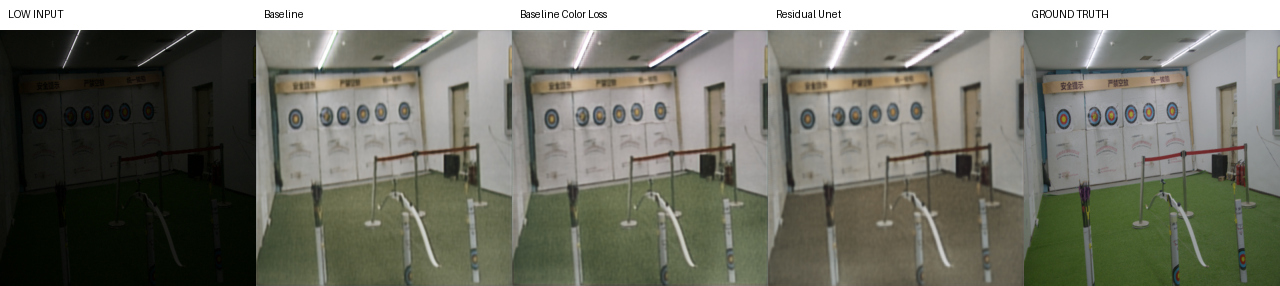
\includegraphics[width=\textwidth]{images/000.png}
\caption{LOL-v2 qualitative comparison. The color-loss model reduces the grayish color cast of the baseline and better preserves the green floor and wall tones, while remaining softer than the ground truth.}
\label{fig:lolv2_qual}
\end{figure*}

\begin{figure*}[!tbp]
\centering
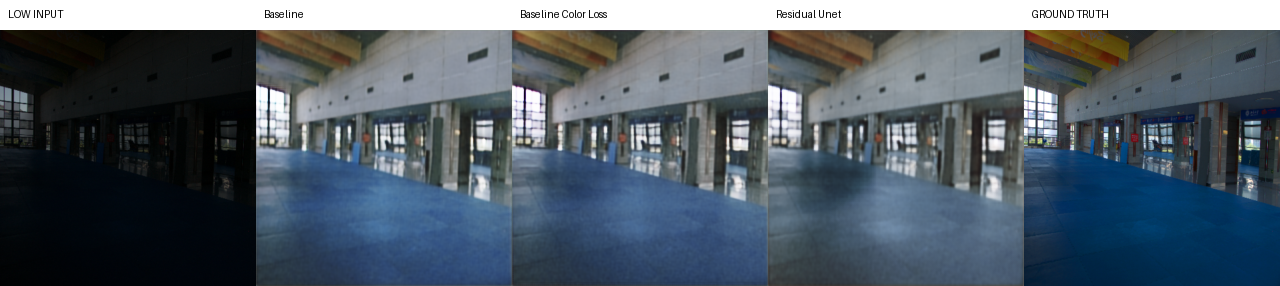
\includegraphics[width=\textwidth]{images/013.png}
\caption{LOL-v1 qualitative comparison. The cross-dataset setting shows that visually plausible enhancement does not always correspond to the highest full-reference scores.}
\label{fig:lolv1_qual}
\end{figure*}

\begin{figure*}[!tbp]
\centering
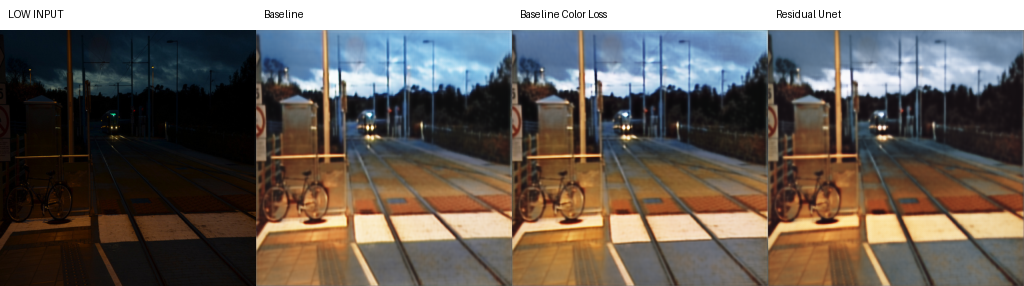
\includegraphics[width=\textwidth]{images/000_bicycle.png}
\caption{ExDark qualitative comparison. Without ground truth, assessment relies on no-reference metrics and visual inspection. ExDark exposes robustness limits because its images differ strongly from LOL-v2 in scene content, noise, and illumination distribution.}
\label{fig:exdark_qual}
\end{figure*}

\subsection{Discussion}
The baseline is competitive as a compact starting point: it brightens images and recovers coarse structure but suffers from over-smoothing and color bias. ResidualUNet provides a useful architectural comparison. It improves in-domain PSNR but degrades cross-dataset full-reference performance, showing that architectural capacity alone is not enough for robust LLIE. The color constancy experiment should be interpreted differently: it is not a new architecture, but a loss-level mitigation applied to the same U-Net baseline. It directly targets color cast and improves no-reference metrics, with only a minor effect on PSNR/SSIM.

The results also show the tension between full-reference and no-reference metrics. On LOL-v1, ResidualUNet has lower PSNR/SSIM than the baseline but better NIQE. Therefore, metric interpretation must be tied to the dataset and visual inspection. PSNR rewards exact target fidelity, while NIQE rewards natural-image statistics. In LLIE, an output can be visually plausible but not pixel-aligned with a specific ground truth exposure.


\section{Model Analysis and Failure Taxonomy}
The models learn a global enhancement mapping: they increase visibility, brighten dark areas, and recover coarse scene structure. However, they do not fully recover high-frequency detail or robustly adapt to all cross-domain illumination statistics. The following taxonomy discusses the main observed failures.

Appendix \ref{app:appendix} summarizes the failures and shows visual examples.

\subsection{Color Cast}
\textbf{Observation.} The baseline often produces outputs that are brighter but slightly grayish or desaturated. In Fig.~\ref{fig:lolv2_qual}, the baseline floor and wall colors are less faithful to the ground truth than the color-loss model.

\textbf{Hypothesis.} L1 and SSIM optimize pixel and structural similarity but do not explicitly constrain global RGB balance. Since many low-light inputs contain weak or biased color information, the model can converge to average-looking colors that reduce reconstruction loss but create a visible cast.

\textbf{Mitigation tested.} The color constancy loss directly penalizes mismatch between predicted and target RGB channel means. It improves NIQE on all datasets and visibly reduces desaturation in the selected LOL-v2 example. This is the main tested mitigation.

\subsection{Halo Artifacts}
\textbf{Observation.} Halo artifacts appear as unnatural bright transitions near high-contrast borders, such as lamps, windows, neon lights, or object silhouettes in dark scenes. They are more likely in ExDark because local light sources are often surrounded by very dark regions.

\textbf{Hypothesis.} The network learns to increase local brightness without an explicit gradient-continuity constraint. Upsampling and skip concatenations can preserve strong edges, but the reconstruction loss may not sufficiently penalize unnatural transition bands.

\textbf{Mitigation proposed.} A gradient-aware loss could penalize discrepancies between Sobel gradients of the prediction and target. This may reduce halos and sharpen transitions, but was not tested in this draft.

\subsection{Over-Smoothing}
\textbf{Observation.} Fine texture is frequently softened. Text, wall details, grass, books, and thin structures become less sharp than in the target. This remains true even when color improves.

\textbf{Hypothesis.} The encoder compresses spatial information, and L1/SSIM favor stable average reconstructions. At $256 \times 256$, some high-frequency details are also lost during resizing. SSIM helps preserve structure but can still accept smooth local patterns.

\textbf{Mitigation proposed.} Edge loss, perceptual loss, or a patch-based high-frequency loss could encourage sharper detail. These were not tested to keep the mitigation focus on color cast.

\subsection{Hallucinated Details}
\textbf{Observation.} Strong hallucinations are limited because the model is trained with supervised reconstruction losses rather than adversarial losses. However, in severely underexposed areas, the prediction can introduce weak false textures or distorted contours not clearly supported by the input.

\textbf{Hypothesis.} When the input signal is nearly absent, the model fills missing information using learned dataset priors. These priors can be plausible but not faithful to the actual target.

\textbf{Mitigation proposed.} Uncertainty-aware evaluation or conservative enhancement in extremely dark regions could reduce unsupported detail synthesis. A denoising-aware or confidence-weighted approach may be useful for future work.

\subsection{Residual Noise}
\textbf{Observation.} Some dark areas remain noisy after enhancement, and some noise becomes more visible because the model brightens low-signal regions. ExDark particularly exposes this limitation.

\textbf{Hypothesis.} The training objective has no explicit noise model. Brightness enhancement and noise amplification are coupled: increasing visibility in dark regions can also increase sensor noise and compression artifacts.

\textbf{Mitigation proposed.} A denoising term, noise-aware augmentation, or training with paired noisy/clean examples could reduce residual noise. BRISQUE degradation on ExDark suggests that this remains an open issue.



\section{Conclusion and Future Work}
This work implements a complete LLIE pipeline with deterministic splits, compact U-Net training, cross-dataset evaluation, visual comparisons, and failure analysis. The baseline establishes a stable reference. The ResidualUNet variant shows that residual blocks improve source-domain PSNR but do not solve generalization. The color constancy mitigation directly addresses color cast, improves no-reference metrics, and produces visibly more faithful colors in qualitative examples.

Future work should first complete the mitigation study suggested by the failure taxonomy. In particular, halo artifacts could be addressed with gradient-aware losses, over-smoothing with edge or perceptual constraints, hallucinated details with confidence-aware enhancement, and residual noise with denoising-aware augmentation or a dedicated noise term. These mitigations were not implemented in the current work, except for color constancy, so they should be evaluated as controlled extensions rather than assumed improvements. A second direction is to test the same mitigation losses on ResidualUNet. This would clarify whether the observed behavior comes mainly from the architecture, from the objective function, or from their interaction under cross-dataset evaluation.

\FloatBarrier

\appendix
\section{Failure Taxonomy Appendix}\label{app:appendix}

Table~\ref{tab:failure_taxonomy_appendix} is a compact index of the failure examples shown in the appendix. For simplicity and consistency, all examples are taken from the U-Net baseline predictions.

\begin{table}[!htbp]
\centering
\caption{Compact index of failure examples.}
\label{tab:failure_taxonomy_appendix}
\small
\footnotesize
\setlength{\tabcolsep}{3pt}
\begin{tabularx}{\columnwidth}{p{0.22\columnwidth}X X p{0.16\columnwidth}}
\toprule
Failure & Main visible effect & Mitigation & Figure \\
\midrule
Color cast & Gray-green, desaturated output. & Color constancy loss, tested. & Fig.~\ref{fig:appendix_color_cast} \\
Halo artifacts & Bright band around local light. & Gradient-aware loss, proposed. & Fig.~\ref{fig:appendix_halo} \\
Over-smoothing & Fine bicycle details become soft. & Edge or perceptual loss, proposed. & Fig.~\ref{fig:appendix_smoothing} \\
Hallucinated details & Distorted hanger contours. & Confidence-aware enhancement, proposed. & Fig.~\ref{fig:appendix_hallucination} \\
Residual noise & Noisy, patchy dark background. & Noise-aware training, proposed. & Fig.~\ref{fig:appendix_noise} \\
\bottomrule
\end{tabularx}
\end{table}

\begin{figure}[!htbp]
\centering
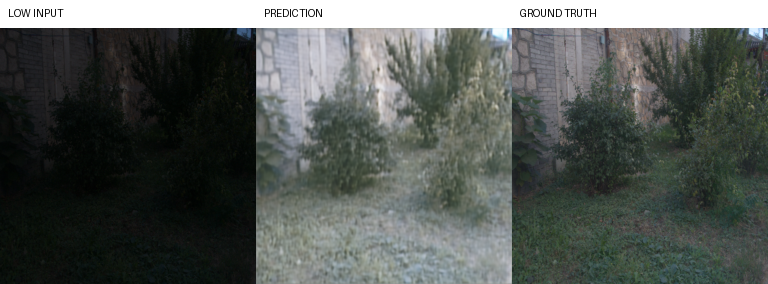
\includegraphics[width=\columnwidth]{images/failure/035.png}
\caption{Color cast example from the U-Net baseline on LOL-v2. The prediction brightens the scene, but vegetation and grass shift toward a gray-green, desaturated appearance compared with the ground truth.}
\label{fig:appendix_color_cast}
\end{figure}

\begin{figure}[!htbp]
\centering
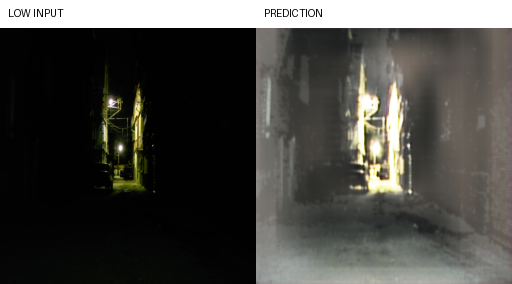
\includegraphics[width=0.95\columnwidth]{images/failure/043_car.png}
\caption{Halo artifact example from the U-Net baseline on ExDark. The local light source is strongly amplified and produces a broad bright halo, creating an unnatural transition between the illuminated area and the surrounding darkness.}
\label{fig:appendix_halo}
\end{figure}

\begin{figure}[!htbp]
\centering
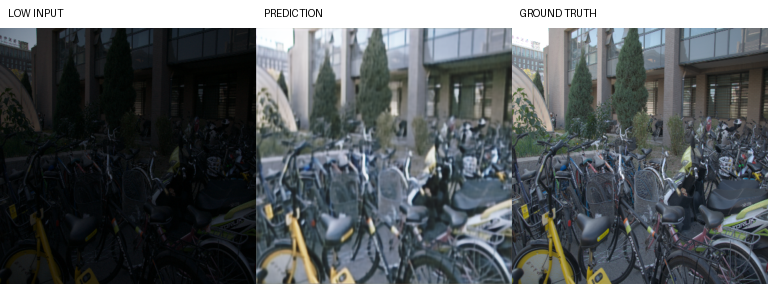
\includegraphics[width=\columnwidth]{images/failure/025.png}
\caption{Over-smoothing example from the U-Net baseline on LOL-v2. The output improves global brightness, but fine bicycle structures such as spokes, handlebars, and overlapping contours become soft and partially merged.}
\label{fig:appendix_smoothing}
\end{figure}

\begin{figure}[!htbp]
\centering
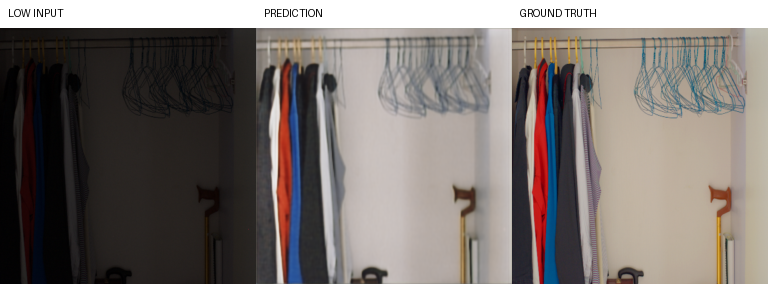
\includegraphics[width=\columnwidth]{images/failure/002.png}
\caption{Hallucinated-detail example from the U-Net baseline on LOL-v1. In the hanger region, thin contours are recovered but several lines appear distorted, merged, or reconstructed in a way that is not fully faithful to the ground truth.}
\label{fig:appendix_hallucination}
\end{figure}

\begin{figure}[!htbp]
\centering
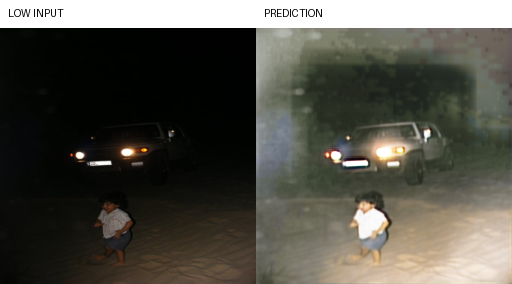
\includegraphics[width=0.95\columnwidth]{images/failure/044_car.png}
\caption{Residual-noise example from the U-Net baseline on ExDark. The prediction reveals the car and foreground, but the dark background becomes noisy and patchy, with visible artifacts amplified by the enhancement.}
\label{fig:appendix_noise}
\end{figure}

\FloatBarrier

\noindent\textbf{Acknowledgements.} This work was developed as an exam project for the Deep Learning course taught by Prof. Vito Walter Anelli at Politecnico di Bari, within the Computer Engineering degree program, Artificial Intelligence and Data Science curriculum. The datasets are not redistributed and remain subject to their original licenses and terms of use.

\begin{thebibliography}{99}

\bibitem{wei2018retinexnet}
C. Wei, W. Wang, W. Yang, and J. Liu,
\newblock ``Deep Retinex Decomposition for Low-Light Enhancement,''
\newblock \emph{British Machine Vision Conference (BMVC)}, 2018.
\newblock Available: \url{https://bmvc2018.org/contents/papers/0451.pdf}.

\bibitem{yang2020semisupervised}
W. Yang, S. Wang, Y. Fang, Y. Wang, and J. Liu,
\newblock ``From Fidelity to Perceptual Quality: A Semi-Supervised Approach for Low-Light Image Enhancement,''
\newblock in \emph{Proceedings of the IEEE/CVF Conference on Computer Vision and Pattern Recognition (CVPR)}, pp. 3060--3069, 2020.
\newblock Available: \url{https://openaccess.thecvf.com/content_CVPR_2020/html/Yang_From_Fidelity_to_Perceptual_Quality_A_Semi-Supervised_Approach_for_Low-Light_CVPR_2020_paper.html}.

\bibitem{loh2019exdark}
Y. P. Loh and C. S. Chan,
\newblock ``Getting to Know Low-Light Images with The Exclusively Dark Dataset,''
\newblock \emph{Computer Vision and Image Understanding}, vol. 178, pp. 30--42, 2019.
\newblock doi: \url{https://doi.org/10.1016/j.cviu.2018.10.010}.

\bibitem{xiang2018resunet}
L. Xiang, Y. Li, W. Lin, Q. Wang, and D. Shen,
\newblock ``Unpaired Deep Cross-Modality Synthesis with Fast Training,''
\newblock in \emph{Deep Learning in Medical Image Analysis and Multimodal Learning for Clinical Decision Support}, LNCS 11045, pp. 155--164, 2018.
\newblock doi: \url{https://doi.org/10.1007/978-3-030-00889-5_18}.

\bibitem{ronneberger2015unet}
O. Ronneberger, P. Fischer, and T. Brox,
\newblock ``U-Net: Convolutional Networks for Biomedical Image Segmentation,''
\newblock in \emph{Medical Image Computing and Computer-Assisted Intervention (MICCAI)}, LNCS 9351, pp. 234--241, 2015.
\newblock doi: \url{https://doi.org/10.1007/978-3-319-24574-4_28}.

\bibitem{wang2004ssim}
Z. Wang, A. C. Bovik, H. R. Sheikh, and E. P. Simoncelli,
\newblock ``Image Quality Assessment: From Error Visibility to Structural Similarity,''
\newblock \emph{IEEE Transactions on Image Processing}, vol. 13, no. 4, pp. 600--612, 2004.
\newblock doi: \url{https://doi.org/10.1109/TIP.2003.819861}.

\bibitem{mittal2013niqe}
A. Mittal, R. Soundararajan, and A. C. Bovik,
\newblock ``Making a `Completely Blind' Image Quality Analyzer,''
\newblock \emph{IEEE Signal Processing Letters}, vol. 20, no. 3, pp. 209--212, 2013.
\newblock doi: \url{https://doi.org/10.1109/LSP.2012.2227726}.

\bibitem{mittal2012brisque}
A. Mittal, A. K. Moorthy, and A. C. Bovik,
\newblock ``No-Reference Image Quality Assessment in the Spatial Domain,''
\newblock \emph{IEEE Transactions on Image Processing}, vol. 21, no. 12, pp. 4695--4708, 2012.
\newblock doi: \url{https://doi.org/10.1109/TIP.2012.2214050}.

\bibitem{loshchilov2019adamw}
I. Loshchilov and F. Hutter,
\newblock ``Decoupled Weight Decay Regularization,''
\newblock in \emph{International Conference on Learning Representations (ICLR)}, 2019.
\newblock Available: \url{https://arxiv.org/abs/1711.05101}.

\bibitem{buchsbaum1980grayworld}
G. Buchsbaum,
\newblock ``A Spatial Processor Model for Object Colour Perception,''
\newblock \emph{Journal of the Franklin Institute}, vol. 310, no. 1, pp. 1--26, 1980.
\newblock doi: \url{https://doi.org/10.1016/0016-0032(80)90058-7}.

\bibitem{krizhevsky2012imagenet}
A. Krizhevsky, I. Sutskever, and G. E. Hinton,
\newblock ``ImageNet Classification with Deep Convolutional Neural Networks,''
\newblock in \emph{Advances in Neural Information Processing Systems (NeurIPS)}, 2012.
\newblock Available: \url{https://proceedings.neurips.cc/paper/2012/hash/c399862d3b9d6b76c8436e924a68c45b-Abstract.html}.

\bibitem{shorten2019augmentation}
C. Shorten and T. M. Khoshgoftaar,
\newblock ``A Survey on Image Data Augmentation for Deep Learning,''
\newblock \emph{Journal of Big Data}, vol. 6, article 60, 2019.
\newblock doi: \url{https://doi.org/10.1186/s40537-019-0197-0}.

\bibitem{he2016resnet}
K. He, X. Zhang, S. Ren, and J. Sun,
\newblock ``Deep Residual Learning for Image Recognition,''
\newblock in \emph{Proceedings of the IEEE Conference on Computer Vision and Pattern Recognition (CVPR)}, pp. 770--778, 2016.
\newblock doi: \url{https://doi.org/10.1109/CVPR.2016.90}.

\end{thebibliography}

\end{document}
